\section{Experiments}
\label{sec:experiments}

We use the SCS interior point solver from CVXPY, which is able to push sparse values arbitrarily close to 0 \cite{cvxpy_sparse_solution}.


\begin{figure}
\centering
\subcaptionbox{Boxplot of $\widehat S_{g}$. \label{fig:boxplot1}}
{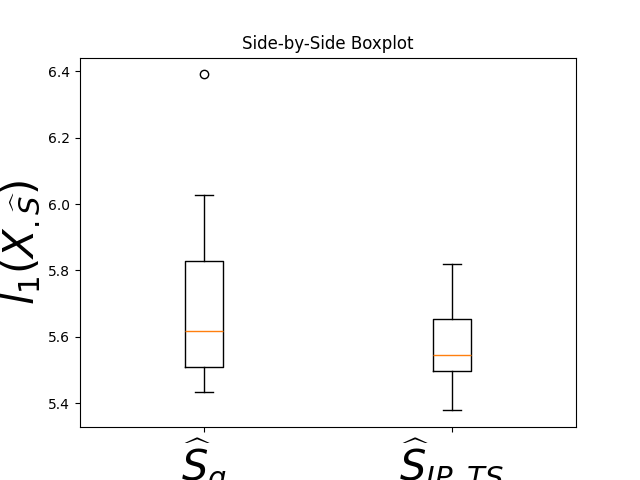
\includegraphics[width=.33\textwidth]{/Users/samsonkoelle/convexlocalisometry/figures/Figure2b.png}}
\subcaptionbox{Boxplot of $\widehat S_{TS}$. \label{fig:boxplot2}}
{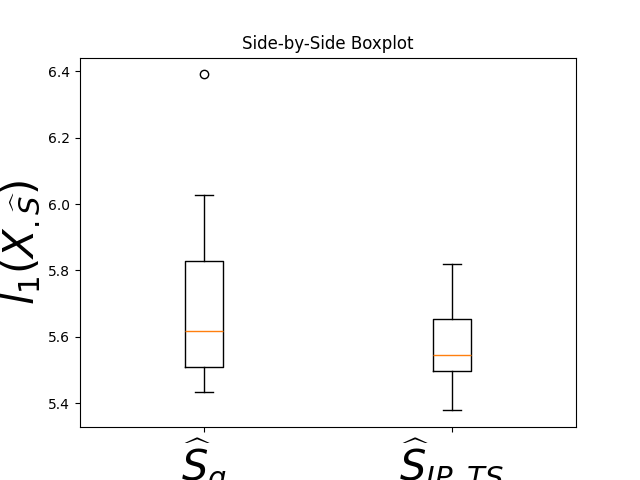
\includegraphics[width=.33\textwidth]{/Users/samsonkoelle/convexlocalisometry/figures/Figure2b.png}}
\subcaptionbox{Boxplot of $\widehat S_{third}$. \label{fig:boxplot3}}
{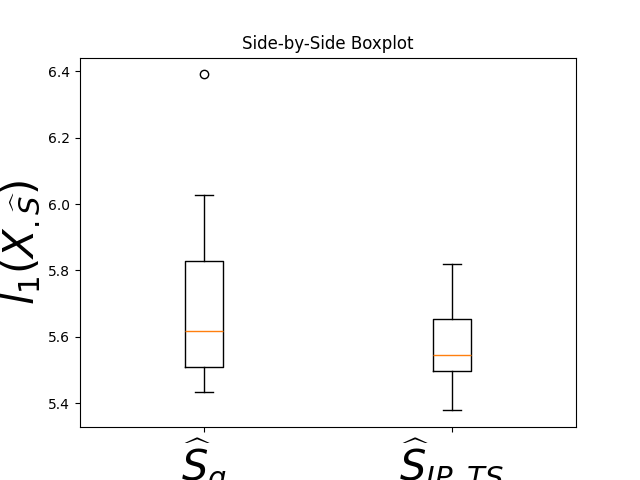
\includegraphics[width=.33\textwidth]{/Users/samsonkoelle/convexlocalisometry/figures/Figure2b.png}}
\caption{Comparison with isometry loss.}
\label{fig:boxplots}
\end{figure}
